% Latex Beamer Template
%
% Copyright 2010 by Frederik Beuth (beuth@hrz.tu-chemnitz.de) - TU-Chemnitz, Dep. for CS, Professorship Artificial Intelligence
%
% Die Vorlage darf frei verwendet werden. Exakt betrifft dies das Latex Beamer Theme und die Sktrut der Vorlage.
% Die Vorlage enthält eine meiner kompletten Präsentation um die Verwendung zu illustrieren.
% Die Inhalte der Präsentation dürfen NICHT frei verwendet werden, daher Frederik Beuth ist immer noch als Author anzusehen.
%
% Benutzung: mittels pdflatex
%
\documentclass[12pt]{beamer}
\mode<presentation>
{
  \usetheme{AIChemnitz}
  \setbeamercovered{transparent}
	% bei Schrittweisem aufdecken sind die noch nicht gezeigten Punkte
	% nur blass dargestellt (nicht ausgeblendet)
}

\usepackage[german]{babel} % lokalisierte Ausgaben
%\usepackage[latin1]{inputenc} % Umlaute direkt eingeben (Editor verwendet Latin-1)
\usepackage[utf8]{inputenc} % Umlaute direkt eingeben (Editor verwendet UTF-8)
\usepackage[T1]{fontenc}    % ??? Umlaute direkt eingeben?
%\usepackage{times}         % Falls die Times schrift verwendet werden soll
\usepackage{textpos}        % um Texte und Bilder absolut zu positionieren

%Falls pdslatex=>dvi=>ps=>pdf benutzt werden soll
%\usepackage[dvips]{graphicx}
%pakete ohne optionen zum schluss laden
\usepackage{
	calc,			% Erweiterung der arithmetischen Funktionen in 
	color,			% im Laufenden Text einfach mit \color{Farbe) zwischen den 
				% Farben umschalten, wobei Farbe einfach 
				% durch z.B. red, blue, black etc. ersetzt wird
				% \textcolor{farbe){Text)
	fancybox,		% shadowbox, doublebox, ovalbox, Ovalbox 
	fancyvrb,		% verbatim Erweiterung:
	float,			% Positionierung von Gleitobjekten genau an der Stelle, wo man
				% 'figure'- oder 'table'-Umgebung die 
				% Positionierung [H] gesetzt werden
	mdwlist,		% compact list: itemize* ..
	tabularx,		% Blocksatzspalten
%eigene packages
	lscape,
	amsmath,		%fuer erweiterte mathe
	bm,			% fuer fette mathe schriften
	xspace,			%mit xspace werden lerrzeichen in makros nicht ignoriert
	subfigure		%fuer sub figures
}

%such Pfad für die Grafiken
\graphicspath{{./images/}}

% Zu Beginn einer Subsection die Gliederung nochmals anzeigen
% (wenn nicht gewünscht einfach rausnehmen)
\AtBeginSubsection[]
{
  \begin{frame}<beamer>
    \frametitle{Gliederung}
    \tableofcontents[currentsection,currentsubsection]
  \end{frame}
}


%
% Grundinformation über die Präsentation
%
\title{TITEL}
% an dieser Stelle funktionieren schon die Overlays! z.B.:
%\title{Titel \only<1,3>{der}\only<2>{{\usebeamercolor[fg]{title frame alerted}der}} Präsentation}
\subtitle{~} % Subtitel, ~ benutzen falls er leer bleiben soll
\author{Frederik Beuth, Fred. H. Hamker}
%\date{\today}
\date{21.10.2010} %Veranstaltungszeit
\occasion{KI2010} %Veranstaltungs Ort

\linespread{1.15} %Zeilenabstand


%
% Verschiedene New-Commands
%
\newcommand{\zb}{z.\,B.~}
\newcommand{\equates}{\mathrel{\widehat{=}}}
%definiert die Anzeige eines neuronalen Areals in den Gleichungen
\newcommand{\Area}[1]{^{\mbox{\tiny #1}}}

%Beispiel für ein neues Kommando mit 2 Parameter, zb.
%\subtexGrafic{0.5}{Overview.jpg} platziert die Grafik 'Overview.jpg' mit 50% der Textbreit
%#1 => Platzhalter für den ersten Parameter, #2 => zweiter Parameter....
\newcommand{\subtexGrafic}[2]{
	\subfigure[#2]{\label{fig:#1}\input{texImg/#1}}
}
%zeigt eine Grafik an
\newcommand{\showGrafic}[2]{
	\begin{center}
		\includegraphics[width=#2\textwidth]{#1}
	\end{center}
}


\begin{document}

%nur für Debug (schaltet incrementelles Aufdecken ab)
%\renewcommand{\pause}{}

% Titelfolie erzeugen
\begin{frame}[plain]
  \titlepage
\end{frame}
%
\section*{Gliederung} 
\begin{frame}
  \frametitle{Gliederung}
  \tableofcontents
\end{frame}
%
\section{Einführung}
%
\begin{frame}
  	\frametitle{Einführung Clusteranalyse}
	\begin{description}

		\item[Aufgabe:]{Erkennung von Gruppen oder Mustern in beliebigen Daten (Mustererkennung)}
		\pause
		\small
		\item[Beispiel:]{Durchführung einer Umfrage über den TV-Konsum\\
			Erkennung von Konsumentengruppen}
	\end{description}
	\begin{minipage}{0.55\textwidth}
		\begin{tabular}{l|c|c|c|c|c}
			Personennummer & 1 & 2 & 3 & 4 & 5 \\
			\hline
			%2d3c datensatz umgemuenzt auf sports, entertainment
			Sport  & 3 & 2 & 8 & 9 & 8 \\
			Entertainment & 1 & 2 & 1 & 0 & 8 \\
			\multicolumn{6}{l}{\hspace{0.5cm}{\small in h pro Woche}}
		\end{tabular}
	\end{minipage}	
\end{frame}
%
\begin{frame}
  \frametitle{Motivation}
  \framesubtitle{Warum Clusteranalyse?}
    \begin{itemize}
	 	 \item Analyseverfahren zur Mustererkennung
	   	 \pause
		 \item Breites Anwendungssprektrum für Clusteranalyseverfahren,\\
			 \zb Bilderkennung, Datamining, Information-Retrieval, \ldots
			\pause 
		 \item Existenz sehr vieler Algorithmen, aber kein perfekter
		 \item Bedarf nach neuen Algorithmen gegeben
  	 \end{itemize}
\end{frame}
%
\begin{frame}
  \frametitle{Motivation}
  \framesubtitle{Warum Default-Artmap?}
  \begin{itemize}
  	 \item Default Artmap: \textbf{A}daptive \textbf{R}esonanz"-\textbf{t}heorie mit überwachtes Clustering (map), Standardverfahren
	 \item Schnelligkeit, gute Resultate, Transparenz, Adaptive Clusteranzahl
		 \pause
 	 \item Entwicklelt von Gail A. Carpenter an der University of Boston, 2003
		 \pause
	 \vskip0.75em
	 \item Neuheit (2003) verursacht ein Problem: \\
	 	Wenig Kenntnisse bezüglich praktischen Einsatzes und Nachteilen des Algorithmus
  \end{itemize}
\end{frame}
%
\begin{frame}
  \frametitle{Ziele der Diplomarbeit}
 \begin{itemize}
	\item Aufbereitung des Algorithmus für künftige Forschung
		\pause
	\item Evalutblendetion des Default Artmap-Verfahrens
		\pause
	\item Nachteile herausarbeiten
 \end{itemize}
\end{frame}
%

\begin{frame}
  	\frametitle{Beispiel Clusteranalyse}
	\small
	\begin{description}
		\item[Aufgabe]{Erkennung von Konsumentengruppen}
	\end{description}
		\pause
	\begin{minipage}{0.60\textwidth}
		\center \textcolor{beamer@tucdark}{\bf Datensatz}
		\vskip1em
		\footnotesize
		\begin{tabular}{l|c|c|c|c|c}
			\textcolor{beamer@tucdark}{\bf Patterns} Nr.    & 1    & 2    & 3   & 4   & 5   \\
			\hline
			%2d3c datensatz umgemuenzt auf sports, entertainment
			Sport in $h$  & 3    &   8  & 8   & 2   & 9   \\
			Entert. in $h$ & 1    & 1    & 8    & 2   & 0   \\
			\hline                                       
			\textcolor{beamer@tucdark}{\bf Merkmal $a_{sport}$}  &0.3  & 0.8  & 0.8 & 0.2 & 0.9 \\
			\textcolor{beamer@tucdark}{\bf Merkmal $a_{entert}$} & 0.1 & 0.1  & 0.8 & 0.2 & 0.0 \\
			\hline                                       
			\textcolor{beamer@tucdark}{\bf Zielklasse $K$} & \color{red} \textbf{0}    & \color{green} \textbf{1} & \color{blue} \textbf{2} & -   & -   \\ 
			Datenmengen		& 
				\multicolumn{3}{c|}{\textcolor{beamer@tucdark}{\bf Trainingsmenge}} & 
				\multicolumn{2}{c}{\textcolor{beamer@tucdark}{\bf Testmenge}}
		\end{tabular}
	\end{minipage}
\end{frame}
%
\begin{frame}
\frametitle{Definitionen für die Clusteranalyse}
	\small
  \begin{description}
  	  	\item[Aufgabe]{Erkennung von Gruppen oder Mustern in beliebigen Daten}
		\item[Rohdaten]{Datenquelle aus der realen Welt}
		\item[Merkmale $M$]{Vorverarbeiteten Rohdaten, erzeugen einen $M$-dim. Merkmalsraum}
		\item[Datensatz]{Zusammenfassung von Merkmalen zu Patterns, Patterns zu Datensätzen}
			\pause
    	\item[Cluster $C$]{Gruppe von Patterns mit ähnlichen Merkmalen}
    	\item[Klasse $L$]{Clustername, mehrere Cluster pro Klasse möglich}
\end{description}
\end{frame}
%
\section{Default Artmap}
%
\begin{frame}
  \frametitle{Gliederung}
  \tableofcontents[currentsection]
\end{frame}
%
\begin{frame}
  	\frametitle{Trainingsalgorithmus}
	\begin{minipage}{0.48\textwidth}
	\begin{itemize}
		\item{Initialisierung: Erstelle aus dem ersten Pattern den ersten Cluster}
		\item{Füge sequentiell Patterns dem jeweils ähnlichsten Cluster hinzu}
		%\item{Oder erstelle einen neuen punktförmigen Cluster}
	\end{itemize}
	\end{minipage}
	\hspace{0.02\textwidth}
	\begin{minipage}{0.48\textwidth}
		\begin{center}
		\vskip0.75em
		Pattern einem Cluster hinzufügen
		\end{center}
		\begin{figure}
		\begin{center}
  				%\input{texImages/sportsInputResonanz}
		\end{center}
		\end{figure}
	\end{minipage}
\end{frame}
%
\begin{frame}
	\frametitle{Trainingsalgorithmus}

	\vskip0.1\textheight
	\begin{center}
		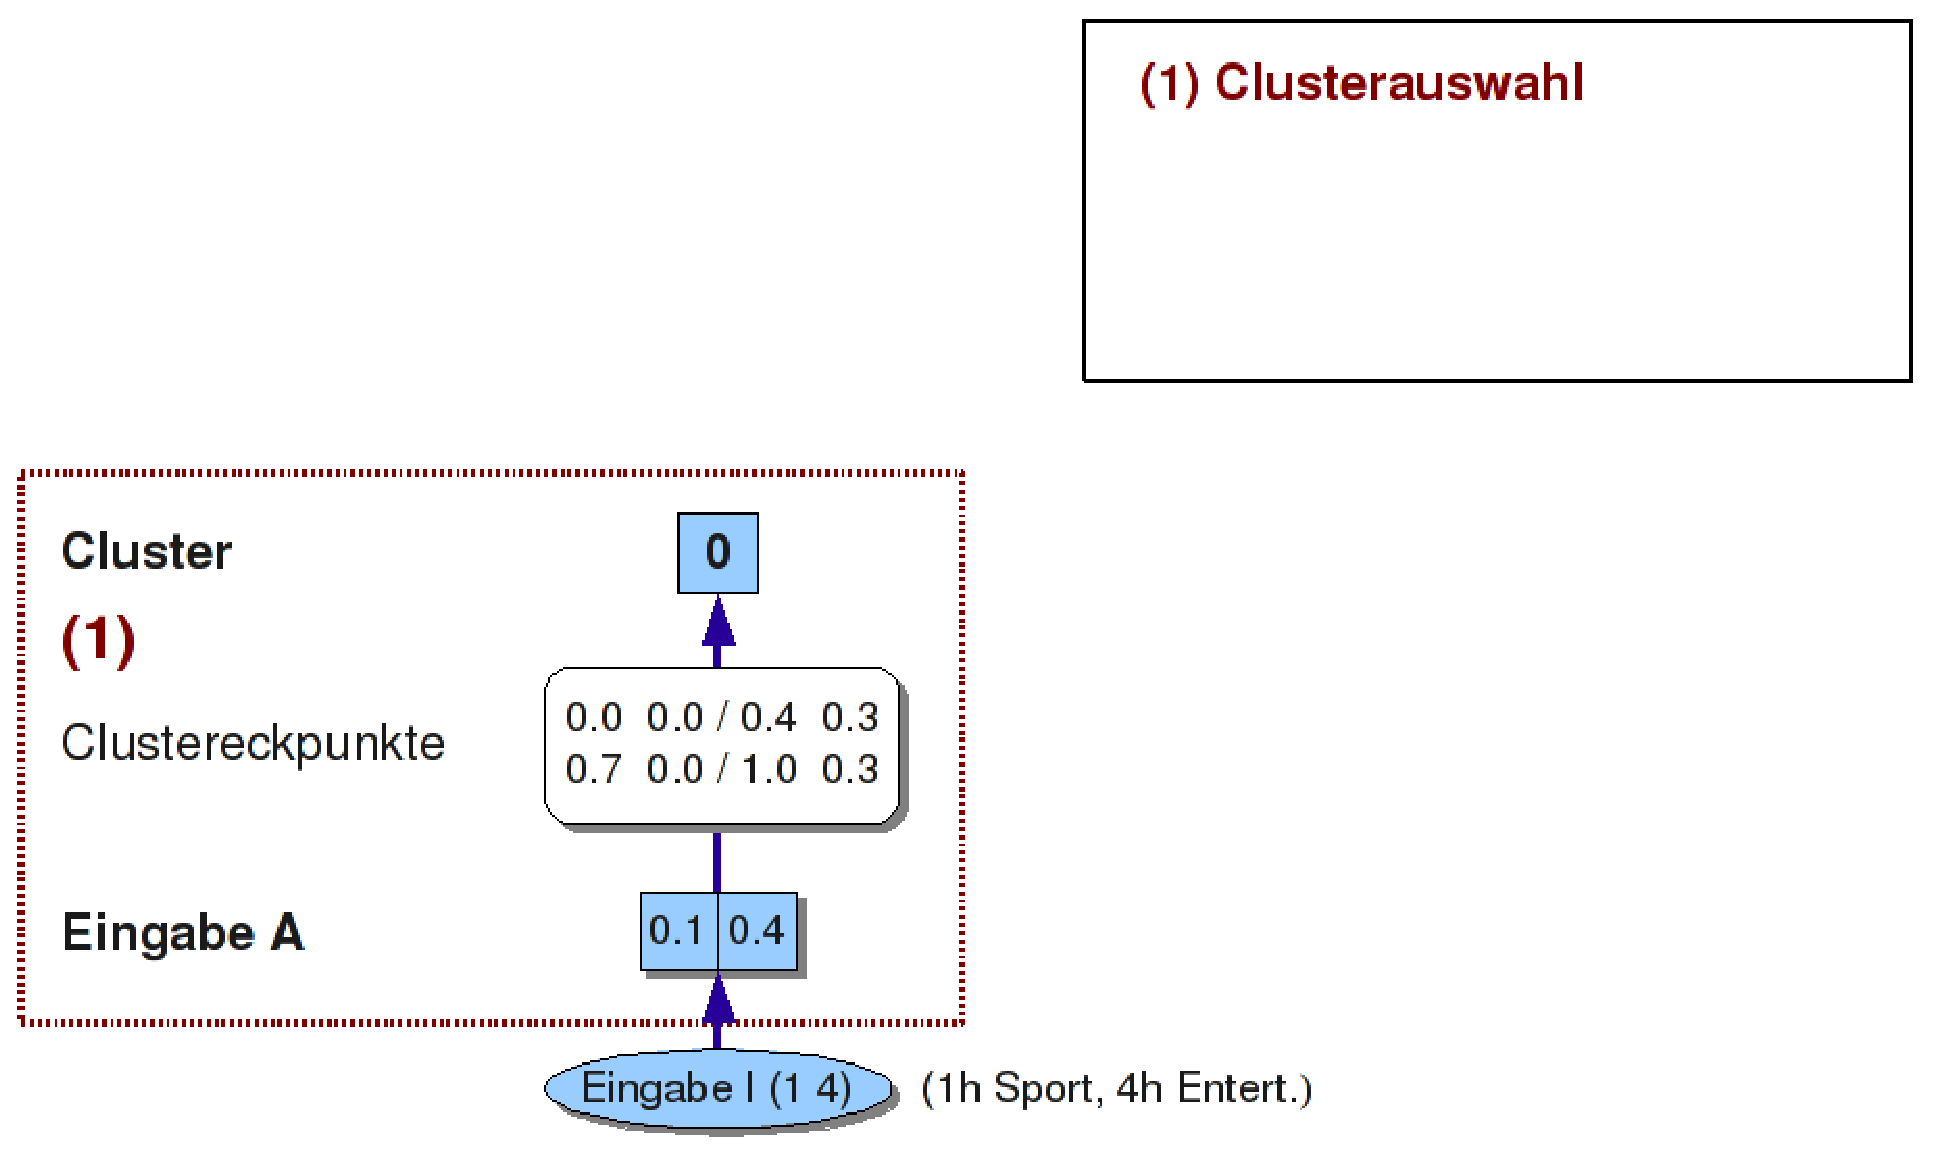
\includegraphics[height=0.9\textheight]{images/artmapBspStep1}
	\end{center}
\end{frame}
\begin{frame}
	\frametitle{Trainingsalgorithmus}

   \addtocounter{framenumber}{-1}
	\vskip0.1\textheight
	\begin{center}
		\includegraphics[height=0.9\textheight]{images/artmapBspStep2Ok}
	\end{center}
\end{frame}
\begin{frame}
	\frametitle{Trainingsalgorithmus}

   \addtocounter{framenumber}{-1}
	\vskip0.05\textheight
	\begin{center}
		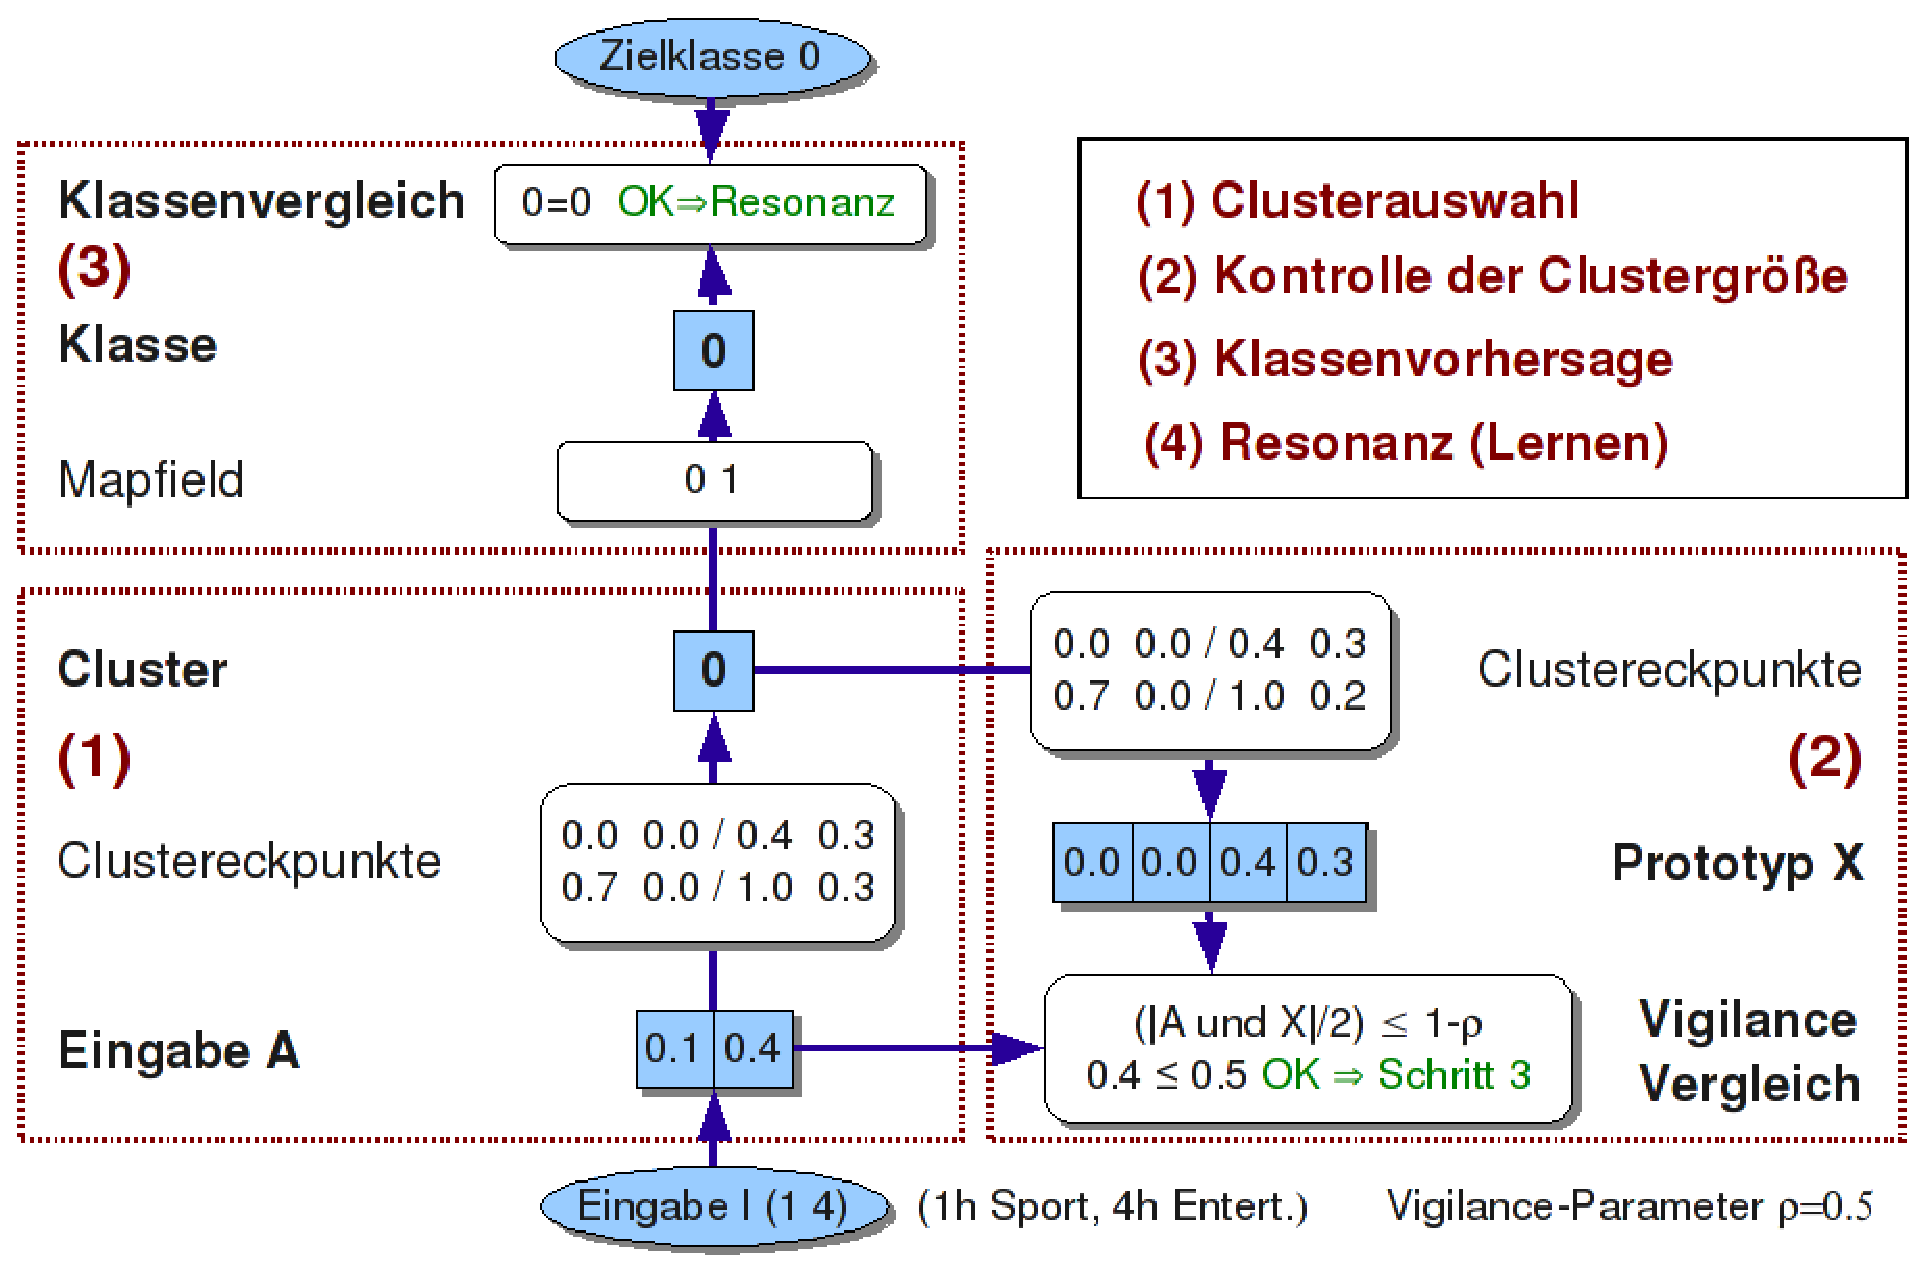
\includegraphics[height=0.95\textheight]{images/artmapBspStep3Ok}
	\end{center}
\end{frame}
%

\section{Evaluation}
%
\begin{frame}
  \frametitle{Gliederung}
  \tableofcontents[currentsection]
\end{frame}
%
\begin{frame}
	\frametitle{Testsetup}
	\begin{description}
		\item[Datensätze]%
			\begin{itemize}%
				\item{Generischer \textbf{2d3c} - Verwendung für Clustervisualisierung}
				\item{\textbf{Iris} Schwertlilien}
				\item{\textbf{Glass} Chemische Elemente von Glas}
			\end{itemize}
			\pause
		\item[Trainiert mit]%
			\begin{itemize}%
				\item Default Artmap
				\item Künstliches Neuronales Netz (KNN) / Back"-pro"-paga"-tion Learning \vskip0.3em
			\end{itemize}
			\pause
		\pause
		\item[Resultate]%
			\begin{itemize}%
				\item Klassifizierungsrate $K = \frac{\mbox{\textit{Korrekte Patterns}}}
					{\mbox{\textit{Gesamtanzahl}}}$ \vskip0.3em
				\item Struktur des Netzes $\#C$ (Anzahl Cluster bzw. Hidden-Neuronen)
			\end{itemize}
\end{description}
\end{frame}

%
\section{Zusammenfassung}
%
\begin{frame}
  \frametitle{Gliederung}
  \tableofcontents[currentsection]
\end{frame}
%
\begin{frame}
  \frametitle<presentation>{Probleme}
	\frametitle{Probleme}
	\begin{itemize}
		\item[--] Geringer Nutzen der Parameteroptimierung
		\item[--] Klassifizierungsrate $K$ ist sehr stark von der Reihenfolge der Patterns im Training abhängig (bis zu $20\%$) 
		\item[ ] Lösung: Eine oder mehrere randomisierte Trainingsmengen, aber dadurch Black-Box Verfahren
	\end{itemize}
\end{frame}
%
\begin{frame}
  \frametitle{Vorteile}
	\begin{itemize}
		\item[+] Bessere Laufzeit als ein KNN
		\item[+] Adaptive Clusteranzahl
  	  	\item[+] Kategorisierungsraten sind gut und vergleichbar mit denen eines KNN
\end{itemize}
\end{frame}
%
\large
\begin{frame}
  \frametitle<presentation>{Zusammenfassung}
%
  % Die Zusammenfassung sollte sehr kurz sein.
	\begin{itemize}
		\item Evaluation: Verfahren ist praktisch einsetzbar
		\item Forschung: Beheben des Problems der Eingabedatenabhängigkeit
\end{itemize}
\end{frame}
%
\LARGE
\begin{frame}
	%Zeigt auf der letzen Folien 'Questions?' an
	%\frametitle{Fragen}
	%\begin{figure}
	%	\begin{center}
	%		Fragen?
	%	\end{center}
	%\end{figure}
	
	%Falls die Arbeit zu einem geförderten Projekt gehört (z.B.:EU, BMBF oder DFG Projekt)
	\begin{figure}
	      \subfigure{\includegraphics[width=0.15\textwidth]{eyeshotsLogo5}} 
	%      \subfigure{\includegraphics[width=0.7\textwidth]{eyeshotsLogoBig}}
	\end{figure}
	\small
	\begin{description}
	  \item [Danksagung:] Diese Arbeit wurde im Rahmen des europäische Projektes ``Self Constructing Hyper Wavelet Algorithms For Extrapolating Linguistics (SCHWAFEL)'' gefördert.	
	\end{description}

\end{frame}

\end{document}
